\documentclass{article}
\usepackage[letterpaper,margin=1in]{geometry}
\usepackage{xcolor}
\usepackage{fancyhdr}
\usepackage{amsmath}
\usepackage{graphicx}
\usepackage{float}

\pagestyle{fancy}

\lhead{\sc \yourname}
\rhead{\sc Physics 142}
\thispagestyle{empty}

\setlength{\parindent}{0cm}
\setlength{\itemindent}{0cm}

\newcommand{\mytitle}{Physics 142: Assignment 3}
\newcommand{\yourname}{Jessica Birky}

\begin{document}
\hrule \vspace{1pt} \hrule 
\begin{center}\Large \textbf{\sc \mytitle} \\
\normalsize \sc Jessica Birky (A13002163)
\end{center}
\hrule \vspace{1pt} \hrule 


% =================================================================================
\bigskip
\textbf{Preliminary Notes:} \\

\textbf{(a)} Error calculation: Error in average energy for energy samples $\chi_{i}$ is computed as 
	\[\langle E\rangle_{T}=\frac{1}{N}\sum_{i=1}^{N} \chi_{i} \pm \frac{\sigma}{\sqrt{N}} \]
	\[\sigma^{2} = \langle \chi_{i}^{2} \rangle - \langle \chi_{i} \rangle^{2} \]

\textbf{(b)} Simulation setup parameters:

\begin{table}[H]
\centering
\begin{tabular}{|l|l|}
	\hline
	Nstep    & Total number of steps computed per walker \\
	Nburn    & Number of samples removed from beginning \\
	Nskip    & Number of steps skipped between data point collection \\
	\hline
\end{tabular}
\end{table}
Nburn and Nskip are implemented to remove the effect of autocorrelation and draw independent samples. So the total number of samples used to compute average and the error for E is N = (Nstep - Nburn)/Nskip. These parameters and other physical constants are defined in setup.cpp. \\

\textbf{(c)} Step size choices: For the classical harmonic oscillator I sample $(x_1, x_2, p_1, p_2)$ using a gaussian distribution with mean 0 and standard deviation 1, using a Box-Muller transformation to draw a gaussian random numbers (X,Y) using uniform distributions $U_1, U_2$ on the interval [0,1]: 
	\[\Theta = 2\pi U_1 \qquad R = \sqrt{-2 ln(U_2)} \]
	\[X = R \cos\Theta \qquad Y = R \sin\Theta \]
For the quantum oscillators I select the step to be -1, 0, or 1, each with equal probability, except when the current value of n=0, then the proposed value will be 0 with 2/3 probability and 1 with 1/3 probability. \\

\textbf{(d)} Numerically determining $\bar{E}(T)$: For determining the relationship between T and $\langle E\rangle$ I use linear regression, for $x=T$, $y=\langle E\rangle$, and $\sigma$ as the error computed as above. Letting $Y = [y_i]$, $A = [1, x_i]$, and C a diagonal matrix with $C_{ii} = \sigma_{i}^{2}$, then solving $Y = AX$ for X gives the slope and intercept:
	\[\begin{bmatrix} b \\ m \end{bmatrix} = X = [A^T C^{-1} A]^{-1} [A^{T} C^{-1} Y] \]

% =================================================================================
\bigskip
\textbf{Question 1}: Electron in a 2D classical harmonic oscillator. 
	\[E = \frac{\vec{p}^2}{2m} + \frac{1}{2}m\omega^2 \vec{r}^2 \]

\textbf{(a)} Determine $\bar{E}(T)$ the thermal average of the energy at temperature T. \\

Notice E can be split up into x and y components:
\begin{align*}
	E &= \frac{\vec{p}^2}{2m} + \frac{1}{2}m\omega^2 \vec{r}^2 
	= \frac{1}{2m}(p_x^2 + p_y^2) + \frac{1}{2}m\omega^2 (x^2 + y^2) \\
	&= \underbrace{\frac{1}{2m}p_x^2 + \frac{1}{2}m\omega^2 x^2}_{E_x} 
	+ \underbrace{\frac{1}{2m}p_y^2 + \frac{1}{2}m\omega^2 y^2}_{E_y}
\end{align*}
So $\langle E \rangle = \langle E_x \rangle + \langle E_y \rangle$. Let's compute for the x direction:
\begin{align*}
	\langle E_x \rangle &= 
	\frac{\int\limits_{-\infty}^{\infty} \int\limits_{-\infty}^{\infty} E_x e^{-E_x/kT} dx \, dp_x}{\int\limits_{-\infty}^{\infty} \int\limits_{-\infty}^{\infty} e^{-E_x/kT} dx \, dp_x} 
	= \frac{\int\int (\frac{p_x^2}{2m} + \frac{1}{2}m\omega^2 x^2) e^{-(\frac{p_x^2}{2m} + \frac{1}{2}m\omega^2 x^2)/kT} dx \, dp_x}{\int\int e^{-(\frac{p_x^2}{2m} + \frac{1}{2}m\omega^2 x^2)/kT} dx \, dp_x}
\end{align*}
For the top integral, the two parts in the sum are:
\begin{align*}
	\int\limits_{-\infty}^{\infty} \int\limits_{-\infty}^{\infty} 
	&\frac{p_x^2}{2m} e^{-(\frac{p_x^2}{2m} + \frac{1}{2}m\omega^2 x^2)/kT} dx \, dp_x
	= \frac{1}{2m} \int\limits_{-\infty}^{\infty} e^{-m\omega^2 x^2/2kT} dx 
	\int\limits_{-\infty}^{\infty} p_x^2 e^{-\frac{p_x^2}{2m}} dp_x \\
	&= \frac{1}{2m} \left[ \sqrt{\frac{2\pi}{m\omega^2 kT}} \right] \left[\sqrt{2\pi} (mkT)^{3/2} \right] 
	= \frac{\pi (kT)^2}{\omega}
\end{align*}

\begin{align*}
	\int\limits_{-\infty}^{\infty} \int\limits_{-\infty}^{\infty} 
	& \frac{1}{2}m\omega^2 x^2 \, e^{-(\frac{p_x^2}{2m} + \frac{1}{2}m\omega^2 x^2)/kT} dx \, dp_x
	= \frac{1}{2}m\omega^2 \int\limits_{-\infty}^{\infty} x^2 \, e^{-m\omega^2 x^2/2kT} dx 
	\int\limits_{-\infty}^{\infty} e^{-\frac{p_x^2}{2m}} dp_x \\
	&= \frac{1}{2}m\omega^2 \left[ \sqrt{2\pi mkT} \right] \left[\sqrt{2\pi} \left(\frac{kT}{m\omega^2}\right)^{3/2} \right] 
	= \frac{\pi (kT)^2}{\omega}
\end{align*}
The top integral is the sum of these two parts, so: 
	\[top = \frac{\pi (kT)^2}{\omega} + \frac{\pi (kT)^2}{\omega} = \frac{2\pi (kT)^2}{\omega}\]
And the bottom integral is:
\begin{align*}
	\int\limits_{-\infty}^{\infty} \int\limits_{-\infty}^{\infty} 
	& e^{-(\frac{p_x^2}{2m} + \frac{1}{2}m\omega^2 x^2)/kT} dx \, dp_x 
	= \int\limits_{-\infty}^{\infty} e^{-m\omega^2 x^2/2kT} dx 
	\int\limits_{-\infty}^{\infty} e^{-\frac{p_x^2}{2mkT}} dp_x  \\
	&= \left[\sqrt{2\pi mkT} \right] \left[\sqrt{\frac{2\pi}{m\omega^2/kT}} \right] 
	= \frac{2\pi kT}{\omega}
\end{align*}
Finally dividing the top and bottom we get $\langle E_x \rangle$:
\[\langle E_x \rangle = \left(\frac{2\pi (kT)^2}{\omega} \right) \left(\frac{\omega}{2\pi kT} \right) = kT \]
Because of symmetry $\langle E_x \rangle = \langle E_y \rangle = kT$, thus the total energy for a partical in a classical harmonic oscillator is
\[\langle E \rangle = \langle E_x \rangle + \langle E_y \rangle = 2kT \]


\textbf{(b)} Design and run a Monte Carlo simulation to numerically determine $\bar{E}(T)$. 

\begin{table}[H]
\centering
\begin{tabular}{|l|l|}
	\hline
	Nstep    & $10^6$ \\
	Nburn    & $10^4$ \\
	Nskip    & $10^3$ \\
	Run time & 205.521 sec \\
	\hline
\end{tabular}
\end{table}

\begin{figure}[H]
\begin{center}
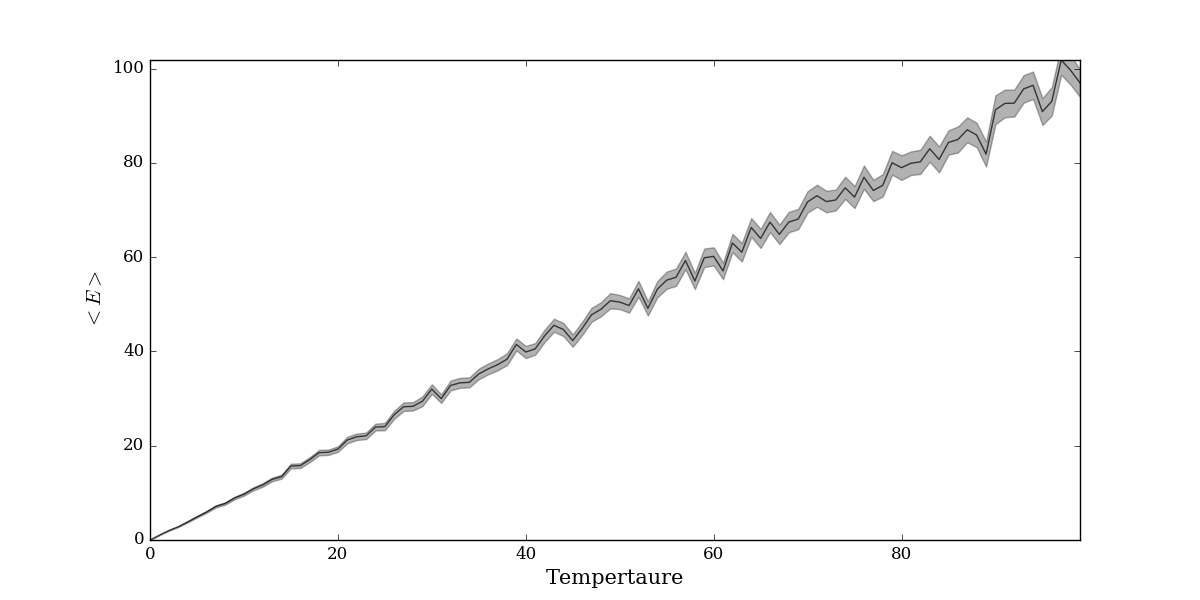
\includegraphics[width=16cm]{../output/classical/expected.png} 
\end{center}
\end{figure}

\begin{figure}[H]
\begin{center}
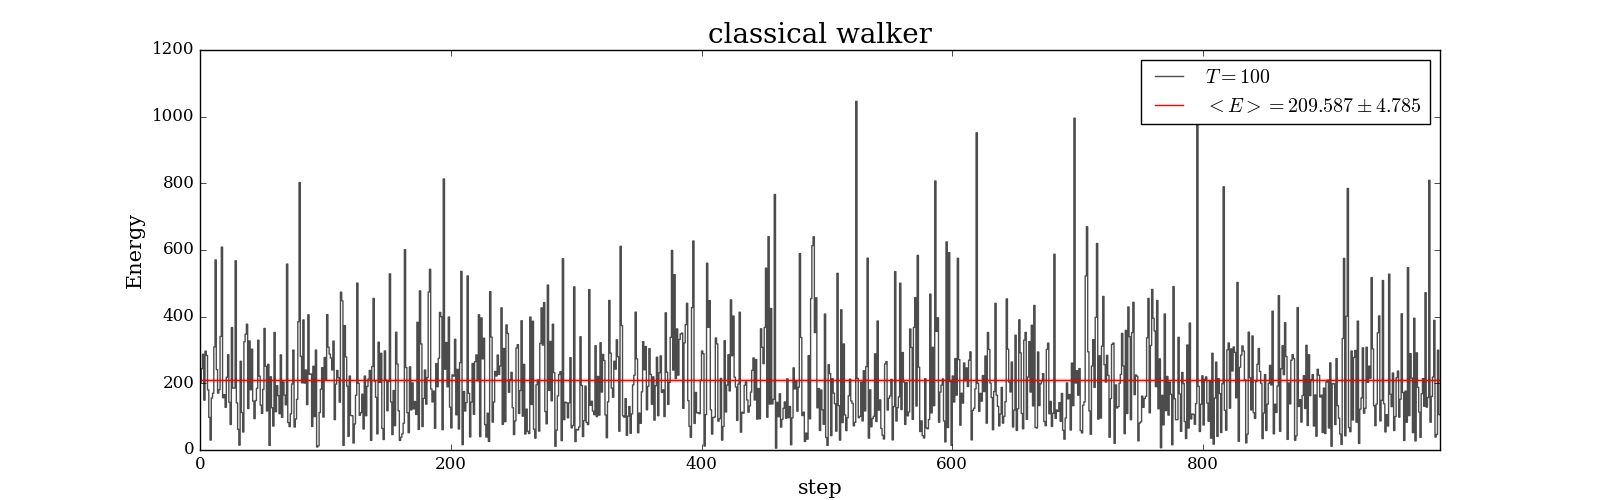
\includegraphics[width=16cm]{../output/classical/walkers.png} 
\end{center}
\end{figure}

Note that the simulaiton yields $\langle E\rangle_{T} \approx 2T$ as expected for $k=1$. \\

\textbf{(c)} Determine $\bar{E}_{2}(T)$. 

\begin{figure}[H]
\begin{center}
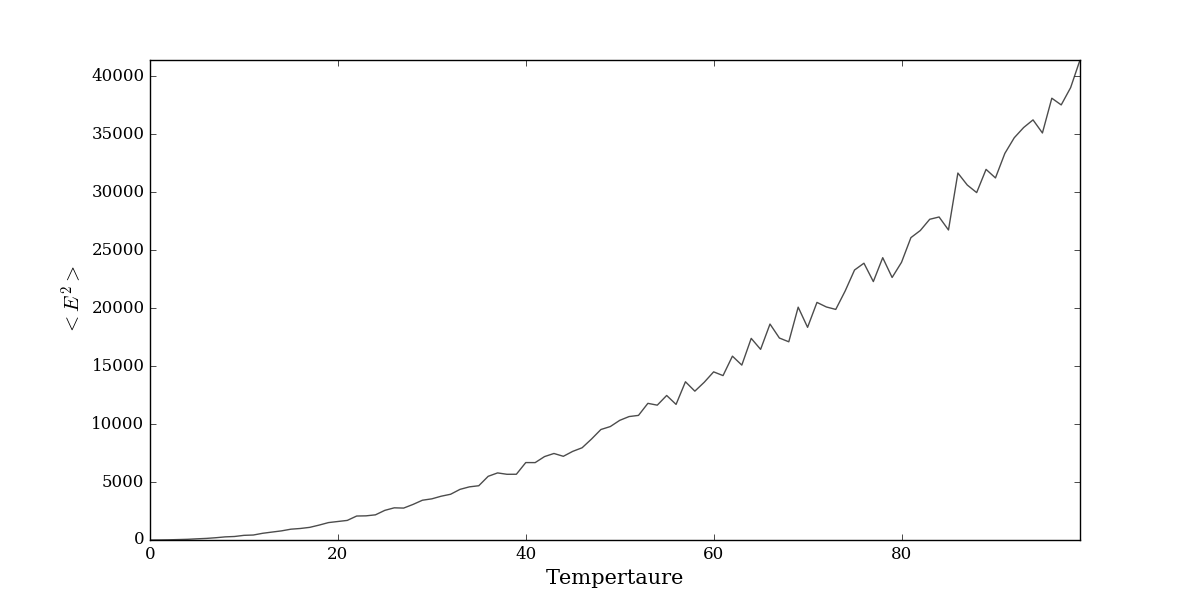
\includegraphics[width=16cm]{../output/classical/expected_sq.png} 
\end{center}
\end{figure}


% =================================================================================
\bigskip
\textbf{Question 2}: Electron in a 1D quantum harmonic oscillator. 
	\[E_{n} = \left(n + \frac{1}{2} \right)\hbar\omega \]

\textbf{(a)} Determine $\bar{E}(T)$ the thermal average of the energy at temperature T. \\

Let $\beta = \frac{\hbar\omega}{kT}$.
\begin{align*}
	\langle E \rangle 
	&= \frac{\sum\limits_{n=0}^{\infty} E_n e^{E_n/kT}}{\sum\limits_{n=0}^{\infty} e^{E_n/kT}}
	= \frac{\sum (n+\frac{1}{2})\hbar\omega \, e^{(n+\frac{1}{2})\hbar\omega/kT}}{\sum e^{(n+\frac{1}{2})\hbar\omega/kT}} \\
	&= \hbar\omega \left[\frac{\sum n e^{-\beta (n+\frac{1}{2})}}{\sum e^{-\beta (n+\frac{1}{2})}} + \frac{ \frac{1}{2} \sum e^{-\beta (n+\frac{1}{2})} }{\sum e^{-\beta (n+\frac{1}{2})}} \right] \\
	&= \hbar\omega \left[\frac{e^{-\beta/2}}{(e^{\beta} - 1)^2} \cdot \frac{(e^{\beta} - 1)}{e^{-\beta/2}} + \frac{1}{2} \right] 
	= \hbar\omega \left[\frac{1}{e^{\beta} - 1} + \frac{1}{2} \right]
\end{align*}
Since $\hbar\omega << kT$, then $\beta << 1$ and we can Taylor series expand $\frac{1}{e^{\beta} - 1} = \frac{1}{\beta} - \frac{1}{2} + O(\beta)$ and get
\begin{equation*}
	\langle E \rangle 
	\approx \hbar\omega \left[\frac{1}{\beta} - \frac{1}{2} + \frac{1}{2} \right]
	= \frac{\hbar\omega}{\beta} = \hbar\omega \left(\frac{kT}{\hbar\omega} \right) = kT
\end{equation*}

\textbf{(b)} Design and run a Monte Carlo simulation to numerically determine $\bar{E}(T)$. \\

\begin{table}[H]
\centering
\begin{tabular}{|l|l|}
	\hline
	Nstep    & $10^8$ \\
	Nburn    & $10^4$ \\
	Nskip    & $10^3$ \\
	Run time & 625.997 sec \\
	\hline
\end{tabular}
\end{table}

\begin{figure}[H]
\begin{center}
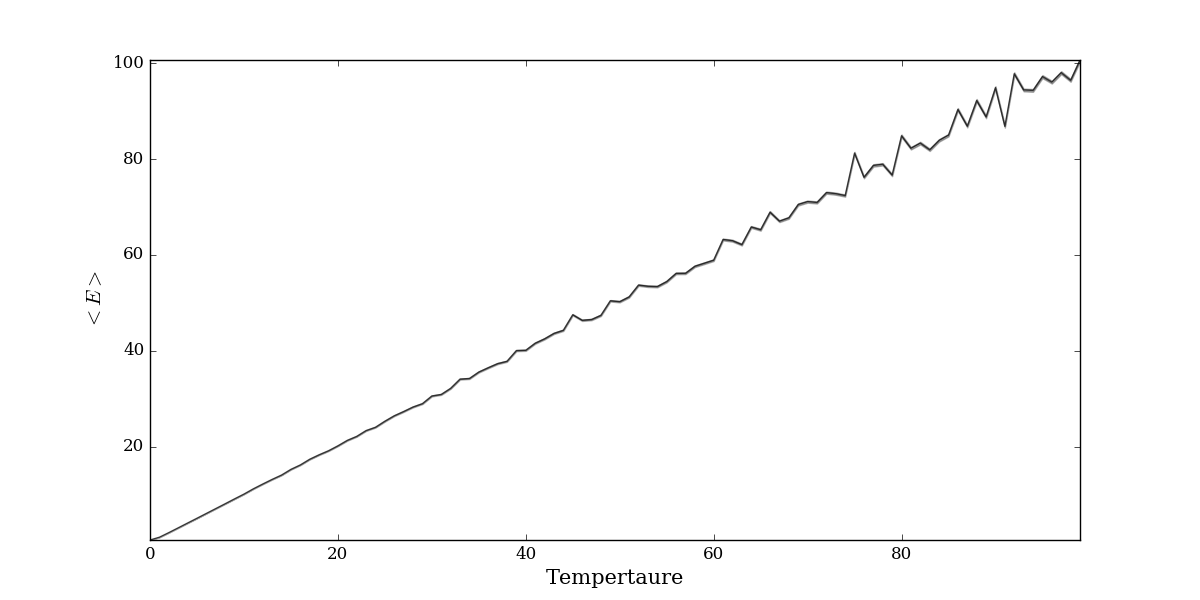
\includegraphics[width=16cm]{../output/quantum/expected.png} 
\end{center}
\end{figure}

\begin{figure}[H]
\begin{center}
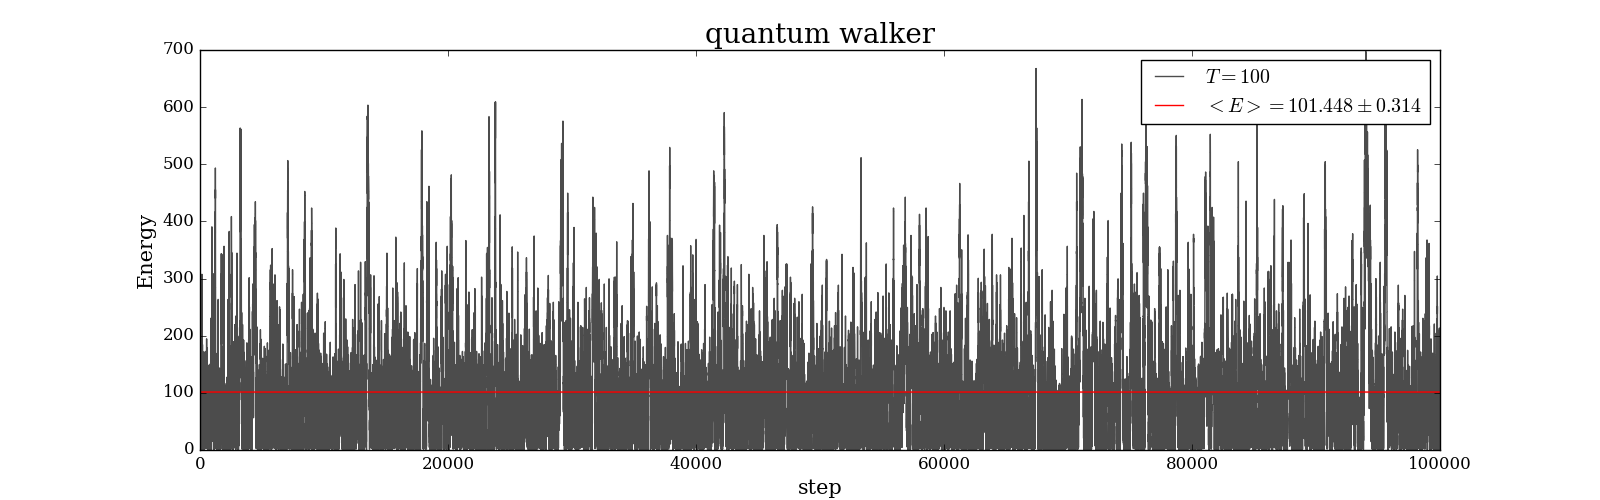
\includegraphics[width=16cm]{../output/quantum/walkers.png} 
\end{center}
\end{figure}

\textbf{(c)} Determine $\bar{E}_{2}(T)$. 

\begin{figure}[H]
\begin{center}
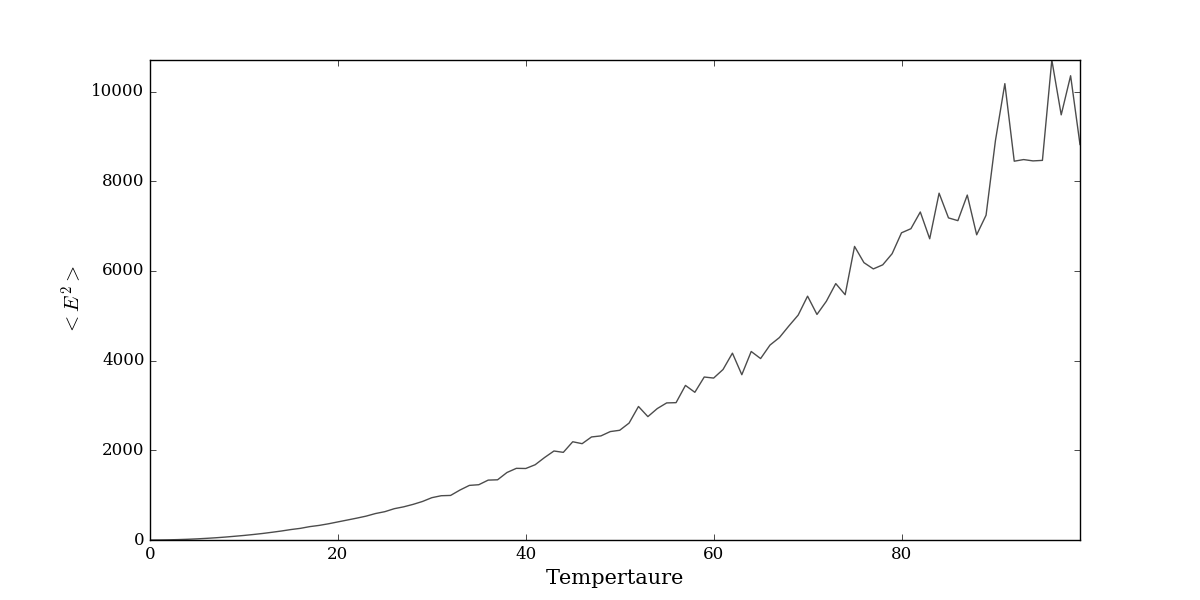
\includegraphics[width=16cm]{../output/quantum/expected_sq.png} 
\end{center}
\end{figure}


% =================================================================================
\bigskip
\textbf{Question 3}: An arbitrary harmonic energy. 
	\[E_{n} = \left(n^2 + \frac{1}{2} \right)\hbar\omega \]

\textbf{(a)} Determine $\bar{E}(T)$ the thermal average of the energy at temperature T. 
\begin{align*}
	\langle E \rangle 
	&= \frac{\sum\limits_{n=0}^{\infty} E_n e^{E_n/kT}}{\sum\limits_{n=0}^{\infty} e^{E_n/kT}}
	= \frac{\sum (n+\frac{1}{2})\hbar\omega \, e^{(n+\frac{1}{2})\hbar\omega/kT}}{\sum e^{(n+\frac{1}{2})\hbar\omega/kT}} \\
	&= \hbar\omega \left[\frac{\sum n^2 e^{-\beta (n^2+\frac{1}{2})}}{\sum e^{-\beta (n^2+\frac{1}{2})}} + \frac{ \frac{1}{2} \sum e^{-\beta (n^2+\frac{1}{2})} }{\sum e^{-\beta (n^2+\frac{1}{2})}} \right] \\
	&= \hbar\omega \left[\frac{\sum n^2 e^{-\beta (n^2+\frac{1}{2})}}{\sum e^{-\beta (n^2+\frac{1}{2})}} + \frac{1}{2} \right]
\end{align*}
Since it is very difficult to evaluate this sum, we can look at the approximation by replacing the sum with an integral:
\begin{align*}
	\langle E \rangle 
	&\approx \hbar\omega \left[\frac{\int\limits_{0}^{\infty} n^2 e^{-\beta (n^2+\frac{1}{2})}}{\int\limits_{0}^{\infty} e^{-\beta (n^2+\frac{1}{2})}} + \frac{1}{2} \right] 
	= \hbar\omega \left[\frac{1}{2\beta} + \frac{1}{2} \right]
	= \frac{\hbar\omega}{2} \left(\frac{kT}{\hbar\omega} \right) + \frac{\hbar\omega}{2}
	= \frac{kT}{2} + \frac{\hbar\omega}{2}
\end{align*}
Now since $kT >> \hbar\omega$, we get
\[\langle E \rangle \approx \frac{kT}{2} \]

\textbf{(b)} Design and run a Monte Carlo simulation to numerically determine $\bar{E}(T)$. \\

\begin{table}[H]
\centering
\begin{tabular}{|l|l|}
	\hline
	Nstep    & $10^7$ \\
	Nburn    & $10^4$ \\
	Nskip    & $10^3$ \\
	Run time & 84.1588 sec \\
	\hline
\end{tabular}
\end{table}

\begin{figure}[H]
\begin{center}
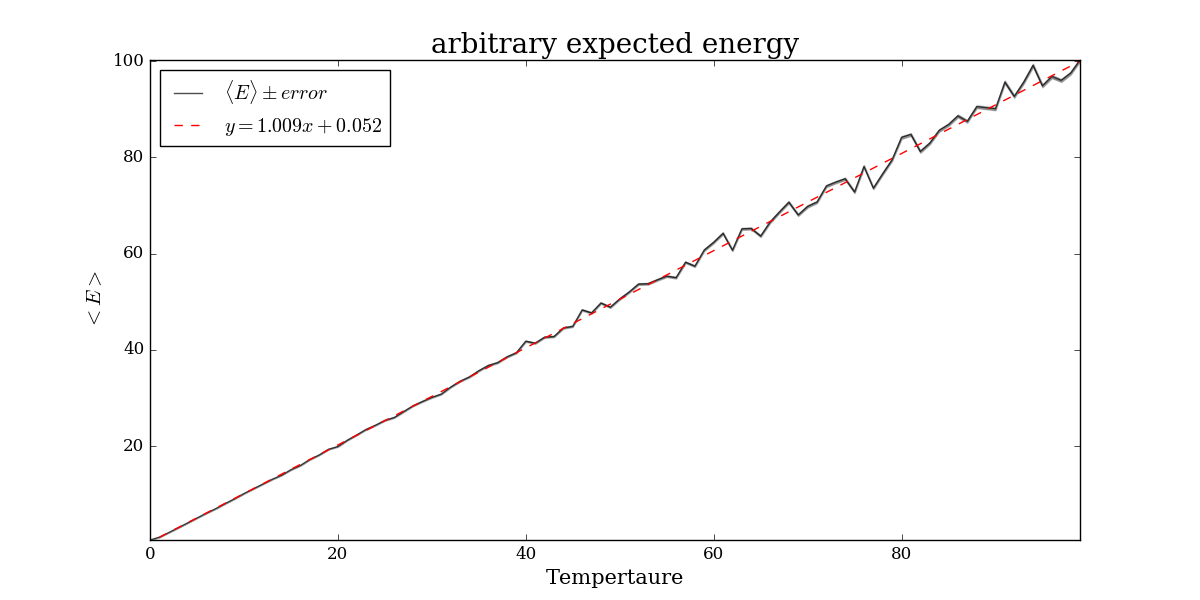
\includegraphics[width=16cm]{../output/arbitrary/expected.png} 
\end{center}
\end{figure}

\begin{figure}[H]
\begin{center}
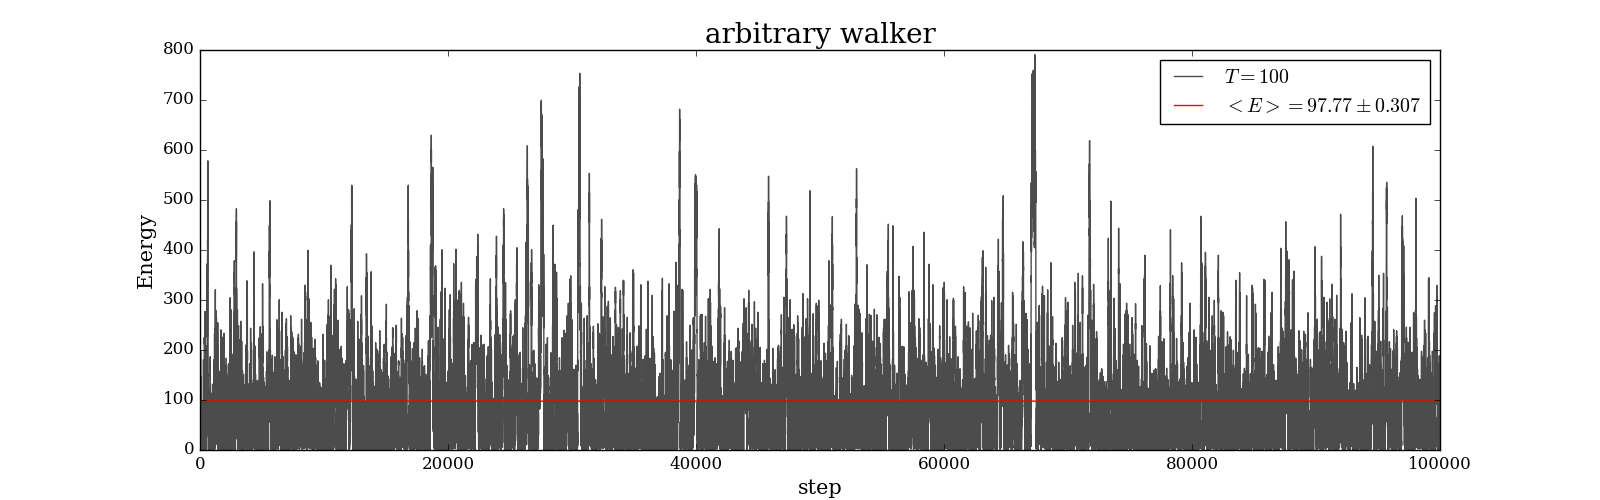
\includegraphics[width=16cm]{../output/arbitrary/walkers.png} 
\end{center}
\end{figure}

\textbf{(c)} Determine $\bar{E}_{2}(T)$. 

\begin{figure}[H]
\begin{center}
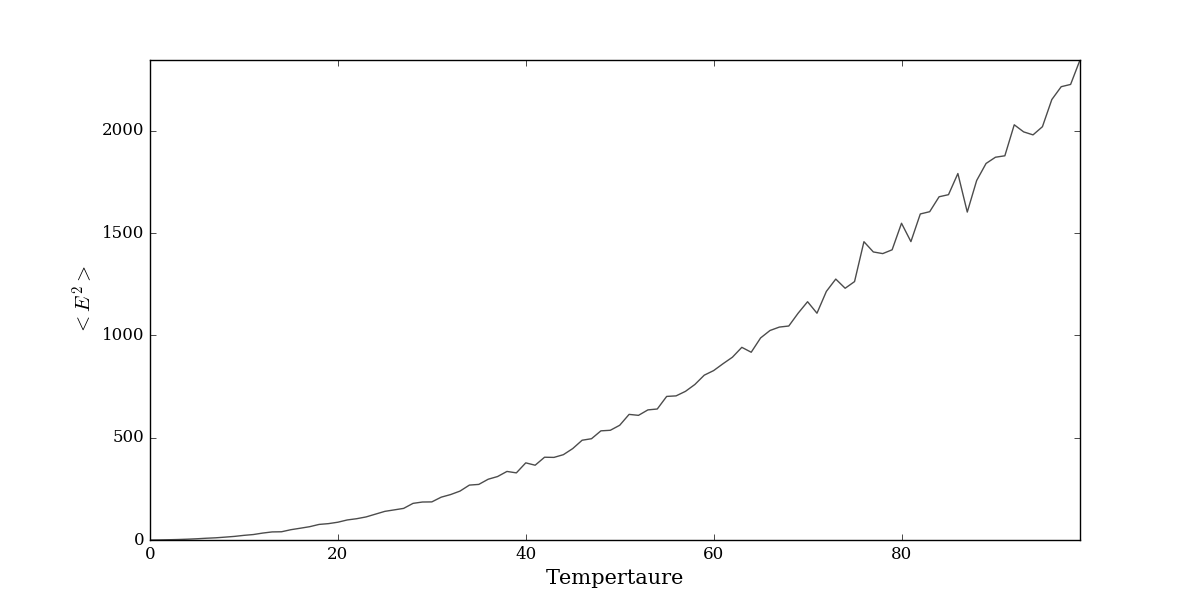
\includegraphics[width=16cm]{../output/arbitrary/expected_sq.png} 
\end{center}
\end{figure}

% =================================================================================
\bigskip
\textbf{Question 4}: Electron in a 2D quantum harmonic oscillator. 
	\[E_{n_1, n_2} = \left(n_1 + \frac{1}{2} \right)\hbar\omega + \left(n_2 + \frac{1}{2} \right)\hbar\omega \]

\textbf{(a)} Determine $\bar{E}(T)$ the thermal average of the energy at temperature T. \\

Since $n_1$ and $n_2$ are sampled independently of each other, the total average energy is the sum of the average energy of $n_1$ plus the average energy of $n_2$, where $\langle E\rangle_{n_1} = \langle E\rangle_{n_1} = kT$ as calculated for the 1D QHO. Thus the average energy for a 2D QHO is:
	\[\langle E\rangle_{T} = \langle E\rangle_{n_1} + \langle E\rangle_{n_2} = kT + kT = 2kT \]

\textbf{(b)} Design and run a Monte Carlo simulation to numerically determine $\bar{E}(T)$. \\

\begin{table}[H]
\centering
\begin{tabular}{|l|l|}
	\hline
	Nstep    & $10^7$ \\
	Nburn    & $10^4$ \\
	Nskip    & $10^3$ \\
	Run time &  296.068 sec \\
	\hline
\end{tabular}
\end{table}

\begin{figure}[H]
\begin{center}
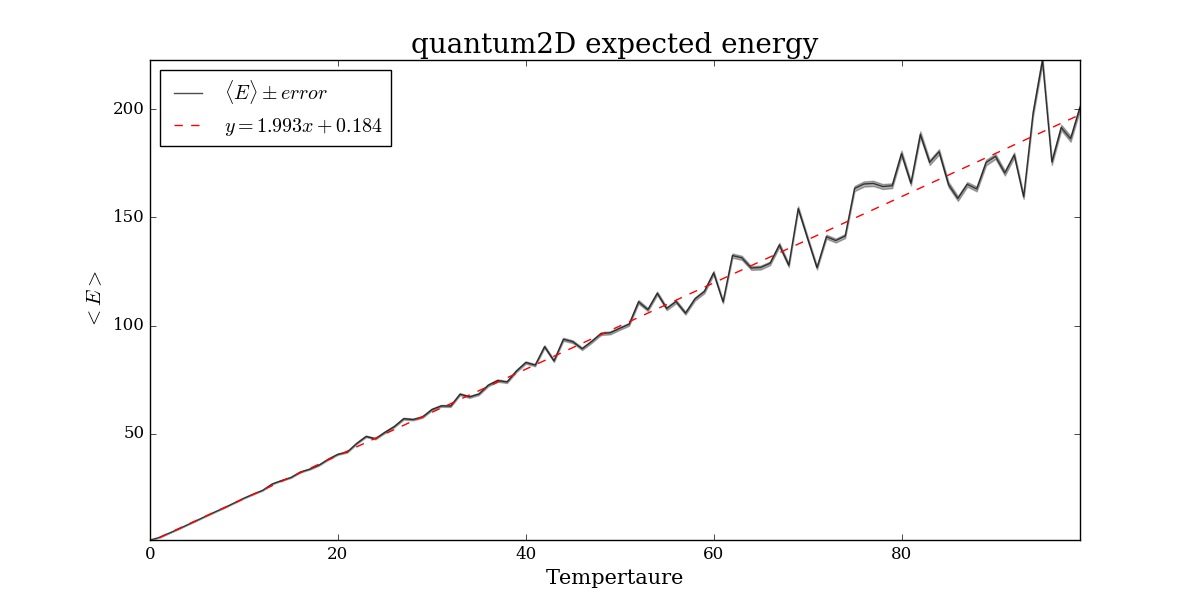
\includegraphics[width=16cm]{../output/quantum2D/expected.png} 
\end{center}
\end{figure}

\begin{figure}[H]
\begin{center}
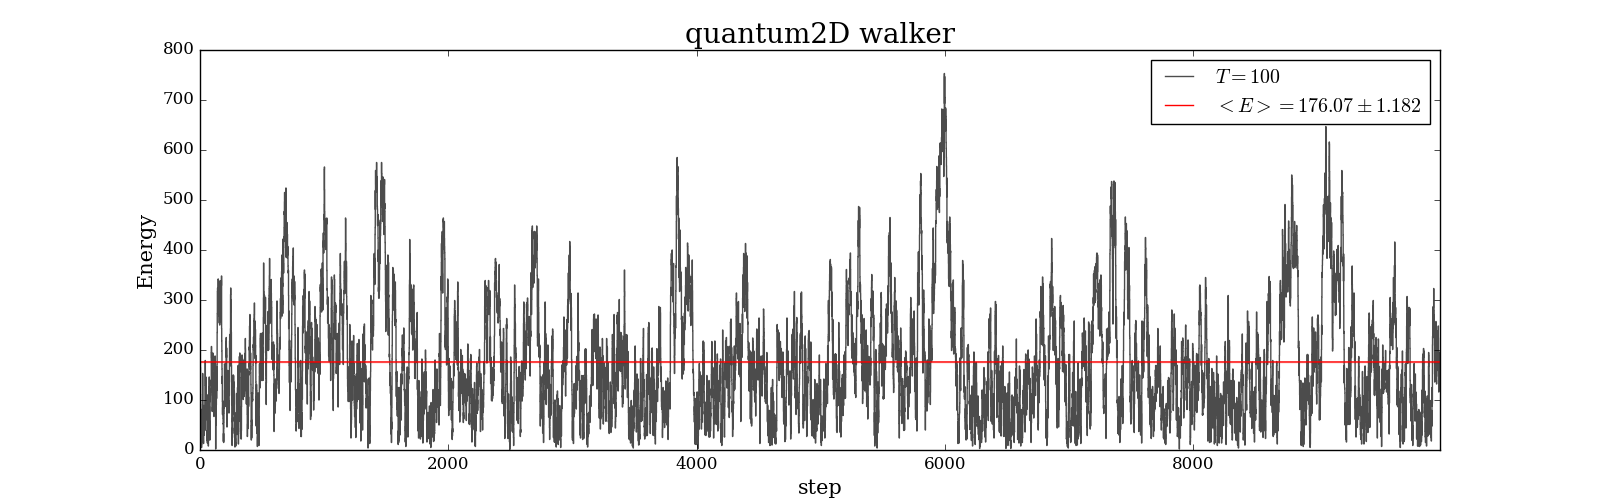
\includegraphics[width=16cm]{../output/quantum2D/walkers.png} 
\end{center}
\end{figure}

\textbf{(c)} Determine $\bar{E}_{2}(T)$. 

\begin{figure}[H]
\begin{center}
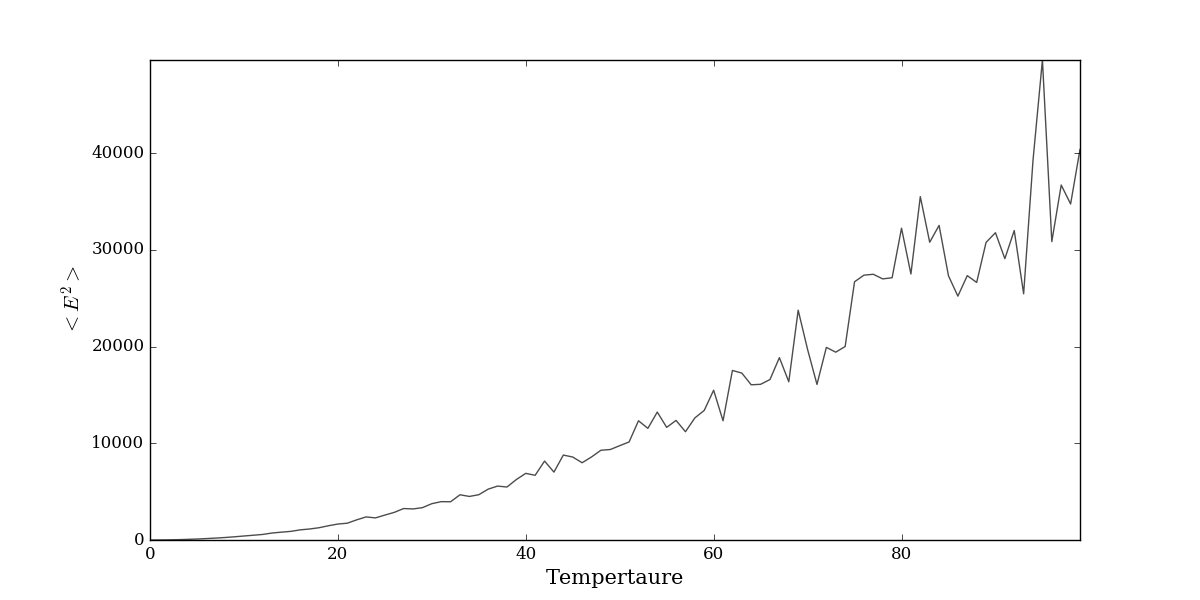
\includegraphics[width=16cm]{../output/quantum2D/expected_sq.png} 
\end{center}
\end{figure}

\end{document}